\documentclass[tikz,border=8pt]{standalone}
\usepackage[utf8]{inputenc}
\usepackage{lmodern}
\usepackage[T1]{fontenc}
\usepackage{amsmath,amssymb}
\usetikzlibrary{shapes.geometric, arrows.meta, positioning, calc, fit, backgrounds}

\definecolor{violetA}{HTML}{6D28D9}
\definecolor{violetB}{HTML}{8B5CF6}
\definecolor{violetC}{HTML}{EDE9FE}
\definecolor{roseA}{HTML}{BE185D}
\definecolor{roseC}{HTML}{FCE7F3}
\definecolor{emeraldA}{HTML}{047857}
\definecolor{emeraldC}{HTML}{D1FAE5}
\definecolor{slateG}{HTML}{475569}
\definecolor{amberA}{HTML}{D97706}
\definecolor{amberC}{HTML}{FEF3C7}

\begin{document}
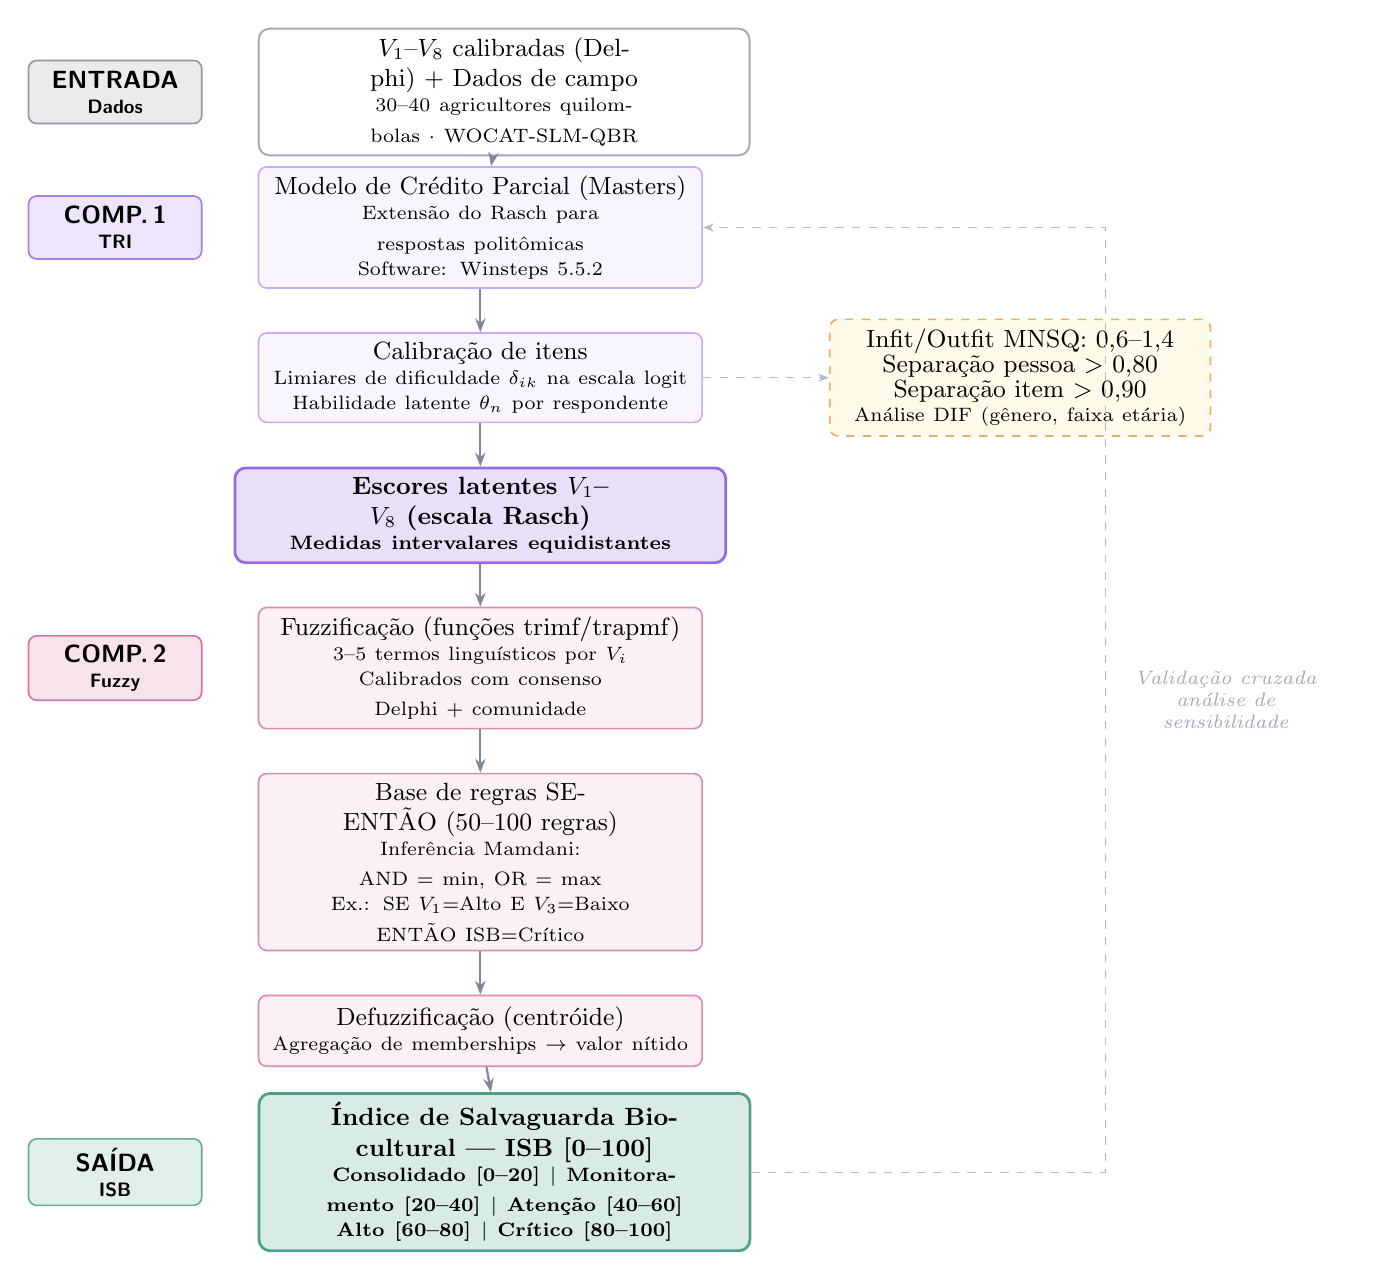
\begin{tikzpicture}[
  phase/.style={
    fill=#1!12, draw=#1!60,
    font=\sffamily\bfseries\small,
    minimum width=2.2cm, minimum height=0.8cm,
    align=center, rounded corners=3pt,
    line width=0.6pt
  },
  mainbox/.style={
    draw=slateG!50, fill=white,
    font=\small, align=center,
    minimum width=6.2cm, minimum height=1.0cm,
    rounded corners=4pt, text width=6.0cm,
    line width=0.7pt
  },
  stepbox/.style={
    draw=#1!50, fill=#1!6,
    font=\small, align=center,
    minimum width=5.6cm, minimum height=0.9cm,
    rounded corners=3pt, text width=5.4cm,
    line width=0.6pt
  },
  metricbox/.style={
    draw=amberA!60, fill=amberC!40,
    font=\small, align=center,
    minimum width=4.8cm, minimum height=0.9cm,
    rounded corners=3pt, text width=4.6cm,
    line width=0.6pt, dashed
  },
  outputbox/.style={
    draw=#1!70, fill=#1!15,
    font=\small\bfseries, align=center,
    minimum width=6.2cm, minimum height=1.0cm,
    rounded corners=4pt, text width=6.0cm,
    line width=1pt
  },
  arr/.style={-{Stealth[length=5pt]}, thick, slateG!70},
  darr/.style={-{Stealth[length=4pt]}, thin, slateG!40, dashed},
  harr/.style={-{Stealth[length=5pt]}, thick, roseA!60},
  node distance=0.55cm
]

%% ═══ ENTRADA ═══
\node[phase=slateG] (ph0) {ENTRADA\\[-2pt]{\scriptsize Dados}};

\node[mainbox, right=0.7cm of ph0] (input)
  {$V_1$--$V_8$ calibradas (Delphi) + Dados de campo\\[-2pt]
   {\scriptsize 30--40 agricultores quilombolas $\cdot$ WOCAT-SLM-QBR}};

%% ═══ COMPONENTE 1 — TRI / RASCH ═══
\node[phase=violetA, below=0.9cm of ph0] (ph1)
  {COMP.\,1\\[-2pt]{\scriptsize TRI}};

\node[stepbox=violetB, right=0.7cm of ph1] (rasch)
  {Modelo de Cr\'edito Parcial (Masters)\\[-2pt]
   {\scriptsize Extens\~ao do Rasch para respostas polit\^omicas}\\[-2pt]
   {\scriptsize Software: Winsteps 5.5.2}};
\draw[arr] (input) -- (rasch);

\node[stepbox=violetB, below=of rasch] (calib)
  {Calibra\c{c}\~ao de itens\\[-2pt]
   {\scriptsize Limiares de dificuldade $\delta_{ik}$ na escala logit}\\[-2pt]
   {\scriptsize Habilidade latente $\theta_n$ por respondente}};
\draw[arr] (rasch) -- (calib);

\node[metricbox, right=1.6cm of calib] (fitm)
  {Infit/Outfit MNSQ: 0{,}6--1{,}4\\[-2pt]
   Separa\c{c}\~ao pessoa $>$ 0{,}80\\[-2pt]
   Separa\c{c}\~ao item $>$ 0{,}90\\[-2pt]
   {\scriptsize An\'alise DIF (g\^enero, faixa et\'aria)}};
\draw[darr] (calib) -- (fitm);

\node[outputbox=violetA, below=of calib] (escores)
  {Escores latentes $V_1$--$V_8$ (escala Rasch)\\[-2pt]
   {\scriptsize Medidas intervalares equidistantes}};
\draw[arr] (calib) -- (escores);

%% ═══ COMPONENTE 2 — FUZZY MAMDANI ═══
\node[phase=roseA, below=0.9cm of ph1 |- escores.south] (ph2)
  {COMP.\,2\\[-2pt]{\scriptsize Fuzzy}};

\node[stepbox=roseA, right=0.7cm of ph2] (fuzz)
  {Fuzzifica\c{c}\~ao (fun\c{c}\~oes trimf/trapmf)\\[-2pt]
   {\scriptsize 3--5 termos lingu\'{\i}sticos por $V_i$}\\[-2pt]
   {\scriptsize Calibrados com consenso Delphi + comunidade}};
\draw[arr] (escores) -- (fuzz);

\node[stepbox=roseA, below=of fuzz] (regras)
  {Base de regras SE-ENT\~AO (50--100 regras)\\[-2pt]
   {\scriptsize Infer\^encia Mamdani: AND = min, OR = max}\\[-2pt]
   {\scriptsize Ex.: SE $V_1$=Alto E $V_3$=Baixo ENT\~AO ISB=Cr\'{\i}tico}};
\draw[arr] (fuzz) -- (regras);

\node[stepbox=roseA, below=of regras] (defuzz)
  {Defuzzifica\c{c}\~ao (centr\'oide)\\[-2pt]
   {\scriptsize Agrega\c{c}\~ao de memberships $\rightarrow$ valor n\'{\i}tido}};
\draw[arr] (regras) -- (defuzz);

%% ═══ SAÍDA — ISB ═══
\node[phase=emeraldA, below=0.9cm of ph2 |- defuzz.south] (ph3)
  {SA\'IDA\\[-2pt]{\scriptsize ISB}};

\node[outputbox=emeraldA, right=0.7cm of ph3] (isb)
  {\'Indice de Salvaguarda Biocultural --- ISB [0--100]\\[-2pt]
   {\scriptsize \textbf{Consolidado} [0--20] $\mid$
    \textbf{Monitoramento} [20--40] $\mid$
    \textbf{Aten\c{c}\~ao} [40--60]}\\[-2pt]
   {\scriptsize \textbf{Alto} [60--80] $\mid$
    \textbf{Cr\'{\i}tico} [80--100]}};
\draw[arr] (defuzz) -- (isb);

%% ═══ RETROALIMENTAÇÃO ═══
\draw[darr] (isb.east) -- ++(4.5,0) |- (rasch.east)
  node[pos=0.25, right, font=\scriptsize\itshape, text=slateG!50, text width=2.8cm, align=center]
  {Valida\c{c}\~ao cruzada\\an\'alise de sensibilidade};

\end{tikzpicture}
\end{document}
